\problemname{Tähtitieteilijä}
\illustration{.3}{img/TychoBrahe.JPG}{}

\noindent
Tähtitieteilijä on intohimoinen tähtien tarkkailija.
Tarkemmin ottaen, häntä miellyttää erityisesti $k$:n~tähden samanaikainen katselu teleskoopinsa avulla.
$r$-säteisen teleskoopin rakentaminen maksa $t\cdot r$~kruunua.
Rakentamisen jälkeen teleskooppi osoittaa tarkalleen origoon $(0,0)$.
Sen suuntaaminen muualle vaatii työtä;
$d$:n~yksikön siirros maksaa $s\cdot d$~kruunua.
Tähtitieteilijä voi tutkia teleskoopilla kaikkia tähtiä, joiden etäisyys teleskoopin osoittamasta pisteestä on enintään $r$.

Kuinka paljon maksaa rakentaa ja suunnata teleskooppi, jonka avulla voi tutkia $k$:ta~tähteä samanaikaisesti?

\medskip

Kaikki koordinaatit ja etäisyydet annetaan euklidisessa tasossa.


\section*{Esimerkki}

Tässä esimerkissä $n=$ tähteä sijaitsee pisteissä $(0,0)$, $(2,0)$ ja $(3,1)$.
% The shaded area shows a telescope of radius~$1$ pointing at $(1,0)$ covering two stars; this costs $s + t$~kroner and is an optimal solution to sample input~$3$.
Väritetty alue näyttää $1$-säteisen teleskoopin, joka osoittaa pisteeseen $(1,0)$ peittäen kaksi tähdistä; tämä maksaa $s + t$~kruunua ja on optimaalinen ratkaisu esimerkkiin~$3$.
% The image also shows optimal solutions to sample inputs~$1$, $2$, and $4$.
Kuvassa näkyy myös optimiratkaisu esimerkkeihin $1$, $2$ ja $4$.

\medskip
\noindent
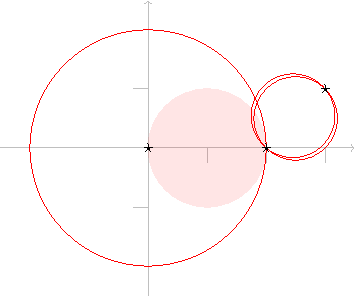
\includegraphics[width=.3\textwidth]{img/samples.pdf}


\section*{Syöte}

% The first line consists of four integers:
Ensimmäisellä rivillä on neljä kokonaislukua:
määrä tähtiä $k$, joita tähtitieteilijä haluaa tutkia samanaikaisesti,
tähtien määrä yön taivaalla $n$,
siirtämishinta~$s$
ja
teleskoopin rakennushinta~$t$.
Seuraa $n$ riviä,
joista $i$:s sisältää $i$:nnen tähden kokonaislukukoordinaatit $x_i$ ja $y_i$.

\section*{Tuloste}

% A single real number: the minimum number of kroner that the astronomer needs to spend.
Yksi reaaliluku: pienin määrä kruunuja, joka tähtitieteilijän tulee käyttää.

\section*{Rajoitteet ja pisteytys} %Constraints and Scoring}

Voit olettaa, että
\begin{enumerate}
\item $1\leq k\leq n\leq 700$. % constraint:kn
\item $x_i, y_i\in \{-10^9,\ldots, 10^9\}$ kaikille $i\in\{1,\ldots,n\}$. % constraint:xy
\item $s,t\in \{0,\ldots, 10^9\}$. % constraint:st
% \item Your output is accepted if it is within a relative or absolute tolerance of $\epsilon = 10^{-6}$ of the correct answer.
\item vastauksesi hyväksytään, jos se on absoluuttisella tai suhteellisella virheellä $\epsilon = 10^{-6}$ päässä oikeasta vastauksesta.
\end{enumerate}


% Your solution will be tested on a set of test groups, each worth a number of points.
Ratkaisu testataan testiryhmillä, joista kullakin on oma pistemäärä.
% Each test group contains a set of test cases.
Jokainen testiryhmä sisältää joukon testitapauksia.
% To get the points for a test group you need to solve all test cases in the test group.
Ryhmän pisteet saa vain, jos ratkaisee kaikki sen testitapaukset.
% Your final score will be the maximum score of a single submission.
Tehtävän lopullinen pistemäärä on suurin yksittäisen lähetyksen pistemäärä.

\medskip
\noindent
\begin{tabular}{lll}
  Ryhmä & Pisteet & Rajoitteet\\\hline
  $1$ & $8$ &  $t\leq s$\\
  $2$ & $9$ & $n\le 50$ and $s=0$\\
  $3$ & $18$ & $s=0$\\
  $4$ & $13$ & $n\leq 50$\\
  $5$ & $14$ & $n\leq 350$\\
  $6$ & $15$ & $\epsilon = 1/10$\\
  $7$ & $23$ & \emph{Ei muita rajoitteita}\\
\end{tabular}
